
\subsection{Kinematik}
Man unterscheidet zwei Arten von Bewegungen:
\begin{itemize}
	\item Translation (geradlinige Bewegung)
	\item Rotation (Drehbewegung)
\end{itemize}

Die meisten Kinematikaufgaben können am einfachsten mit einem v-t Diagramm gelöst werden. Die Fläche unter der Kurve stellt die Geschwindigkeit dar. Die Steigung der Kurve ist die Beschleunigung.

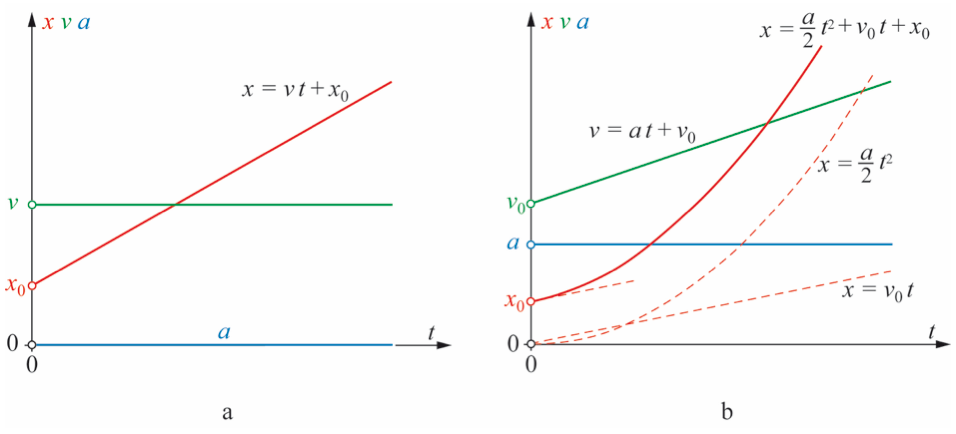
\includegraphics[width=0.7\linewidth]{images/kinematik}

\subsubsection{Translation}
\begin{tabbing}
	\begin{tabu} to \linewidth {X l l}
		\toprule
		Art & Geschwindigkeit v & Beschleunigung a \\
		\midrule
		gleichförmig & konstant & 0 \\
		gleichmässig beschleunigt & ändert sicht gleichmässig & konstant \\
		ungleichmässig beschleunigt & ändert sich ungleichmässig & ändert sich \\
	\end{tabu}
\end{tabbing}


\paragraph{Konstante Geschwindigkeit (gleichförmig)}

\begin{tabbing}
	\begin{tabu} to \linewidth {l X l X l X}
		\toprule
		Geschwindigkeit & $v = \frac{s}{t}$ &
		Strecke & $s = v \cdot t + s_0$ &
		Zeit & $t = \frac{s}{v}$ \\
		\bottomrule
	\end{tabu}
\end{tabbing}

\paragraph{Konstante Beschleunigung (gleichmässig)}

\begin{tabbing}
	\begin{tabu} to \linewidth {l X X}
		\toprule
		& Ohne Anfangsgeschwindigkeit & Mit Anfangsgeschwindigkeit \\
		\midrule
		Beschleunigung & 
		$a = \frac{\Delta v}{ \Delta t} = \dfrac{v^2}{2s} = \dfrac{2s}{t^2}$ &
		$a = \frac{v^2 - v_0^2}{2s}$ \\
		Geschwindigkeit & 
		$v = a \cdot t = \sqrt{2 a s}$ &
		$v = \sqrt{2a(s-s_0) + v_0^2} = a \cdot t + v_0 $ \\
		$\varnothing$ Geschwindigkeit & 
		$v_m = \frac{v_1 + v_2}{2} = \frac{at}{2} = \frac{s}{t}$ &
		 \\
		Strecke & 
		$s = \frac{v t}{2} = \frac{a t^2}{2} = \frac{v^2}{2a}$ &
		$s = \frac{1}{2} at^2 + v_0 t + s_0 = \frac{v^2 - v_0^2}{2a} $ \\
		Zeit & 
		$t = \frac{v}{a} = \sqrt{\frac{2s}{a}}$ & \\		
	\end{tabu}
\end{tabbing}

\begin{tabbing}
	\begin{tabu} to \linewidth {l X l}
		Variable & Bedeutung & SI-Einheit \\
		\midrule
		$v$ & Geschwindigkeit  & $\frac{m}{s}$ \\ 
		$a$ & Beschleunigung  & $\frac{m}{s^2}$ \\ 
		$t$ & Zeit  & $s$ \\ 
		$s$ & Strecke  & $m$ \\ 
		\bottomrule
	\end{tabu}
\end{tabbing}
\subsubsection{Rotation}

\begin{itemize}
	\item Eine Rotation heisst gleichförmig, wenn die Winkelgeschwindigkeit $\omega$ konstant ist. 
	\item Die Tangentialgeschwindigkeit ($\vec{v}=\omega r$) ist die Geschwindigkeit die in der Rotation gerade aus geht
\end{itemize}

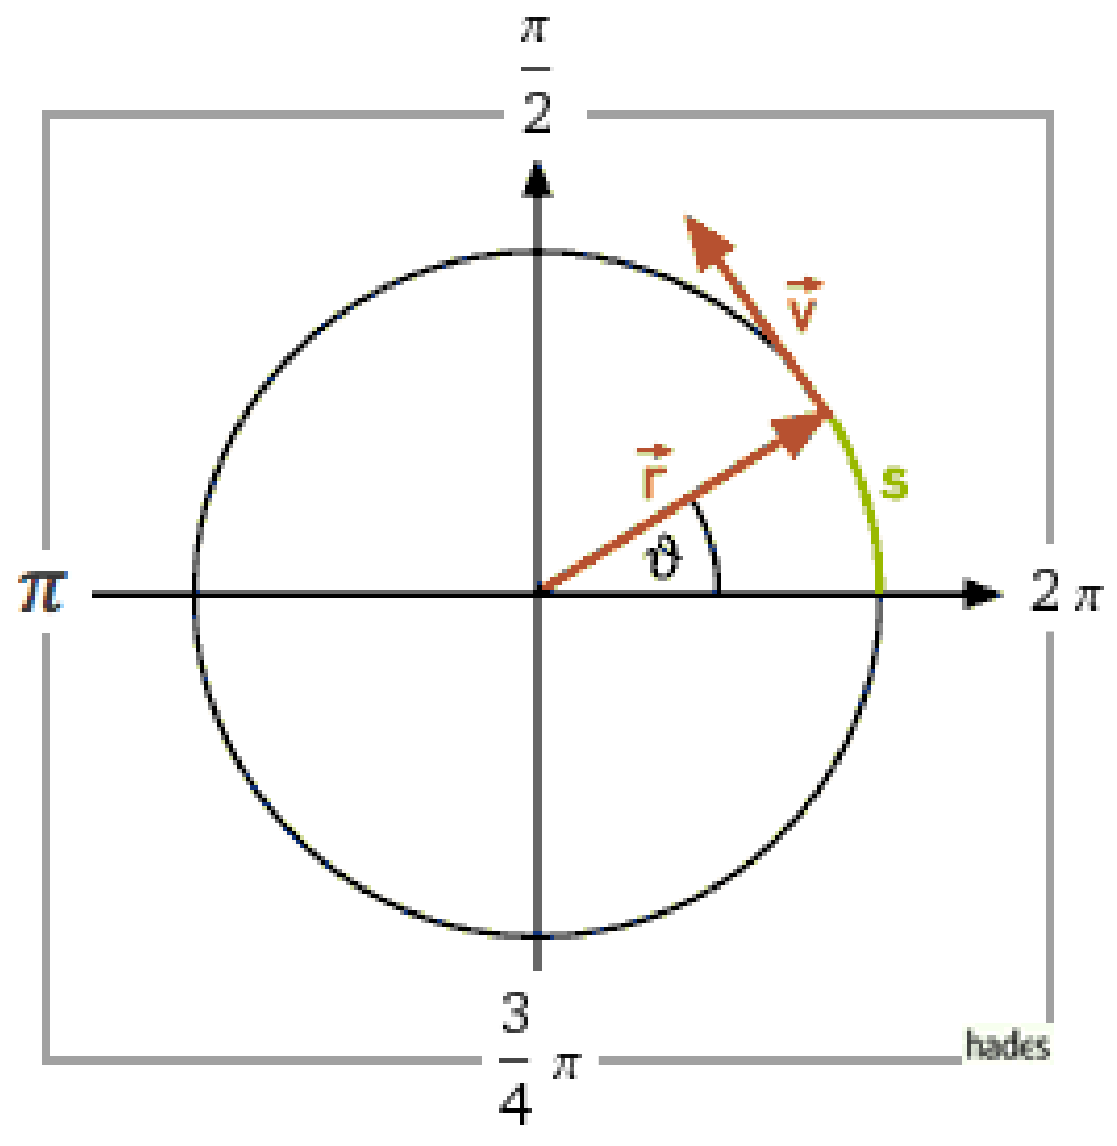
\includegraphics[width=0.2\linewidth]{images/rotation}

\paragraph{Konstante Geschwindigkeit (gleichförmig)}

\begin{tabbing}
	\begin{tabu} to \linewidth {l X l X}
		\toprule
		Winkelgeschwindigkeit & $\omega = \frac{\varphi}{t} = 2 \pi f$ &
		Rotationswinkel & $\varphi = \omega \cdot t$ \\
		Zeit & $t = \frac{\varphi}{\omega}$ &
		Drehzahl & $n = \frac{z}{t} = \frac{1}{T} = \frac{\omega}{2 \pi}$  \\
		Periodendauer & $T = \frac{1}{n} = \frac{2\pi r}{v} = \frac{2\pi}{\omega}$ &
		Anz. Umdrehungen & $N = \frac{\varphi}{2 \pi}$ \\
		\bottomrule
	\end{tabu}
\end{tabbing}

\paragraph{Konstante Beschleunigung (gleichmässig)}

\begin{tabbing}
	\begin{tabu} to \linewidth {l X X}
		\toprule
		& Ohne Anfangsgeschwindigkeit & Mit Anfangsgeschwindigkeit \\
		\midrule
		Winkelbeschleunigung & 
		$\alpha = \frac{\omega}{t} = \frac{2 \varphi}{t^2} = \frac{\omega^2}{2 \varphi}$ &
		$\alpha = \frac{\omega^2 - \omega_0^2}{2 \varphi}$ \\
		Winkelgeschwindigkeit & 
		$\omega = \alpha t = \sqrt{2 \alpha \varphi}$ &
		$\omega = \alpha t + \omega_0 = \sqrt{2\alpha \varphi + \omega_0^2} $ \\
		$\varnothing$ Winkelgeschwindigkeit & 
		$\omega_m = \frac{\alpha t}{2} = \frac{\varphi}{t}$ & \\
		Rotationswinkel & 
		$\varphi = \frac{\omega t}{2} = \frac{\omega^2}{2 \alpha} = \frac{\alpha t^2}{2} = \frac{s}{r} = 2\pi N$ &
		$\varphi = \frac{(\omega_0 + \omega_1)t}{2} = \frac{\omega^2 - \omega_0^2}{2 \alpha} = \frac{\alpha t^2}{2} + \omega_0 t + \varphi_0$ \\
	\end{tabu}
\end{tabbing}

\paragraph{Umrechnung Translation und Rotation}

\begin{tabbing}
	\begin{tabu} to \linewidth {l X l X l X}
		\toprule
		Geschwindigkeit & $v = r \cdot \omega$ &
		Beschleunigung & $a = r \cdot \alpha$ &
		Strecke & $s = r \cdot \varphi$ \\
		Winkelgeschwindigkeit & $\omega = \frac{v}{r}$ &
		Winkelbeschleunigung & $\alpha = \frac{a}{r}$ &
		Rotationswinkel & $\varphi = \frac{s}{r}$ \\
		\bottomrule
	\end{tabu}
\end{tabbing}

\begin{tabbing}
	\begin{tabu} to \linewidth {l X l}
		Variable & Bedeutung & SI-Einheit \\
		\midrule
		$\varphi$ & Rotationswinkels  & rad (Bogenmass) \\ 
		$\omega$ & Winkelgeschwindigkeit & $\frac{rad}{s}$ \\
		$\alpha$ & Winkelbeschleunigung & $\frac{rad}{s^2}$ \\
		$n = f$ & Drehzahl rsp. Umdrehungsfrequenz & $\frac{1}{s} = Hz$ \\
		$N$ & Anzahl ausgeführte Umdrehungen & \\
		$T$ & Periodendauer, Umlaufdauer & $s$ \\
		$t$ & Zeit die für die Drehung um den Winkel $\varphi$ benötigt wird & $s$ \\
		$s$ & Weg beim Umfang & $m$ \\
		$r$ & Radius & $m$ \\
		$z$ & Anzahl der Umdrehungen während der Zeit t & \\
		\bottomrule
	\end{tabu}
\end{tabbing}

\paragraph{Translation vs. Rotation}
\begin{tabbing}
	\begin{tabu} to \linewidth {l|l|l||l|l|l}
		\toprule
		& Translation & &  & Rotation &  \\ 
		\midrule
        S & Grösse & Beziehung & S & Grösse & Beziehung \\
        \midrule
        $s$ & Weg [$m$] & - & $\phi$ & Winkel [$rad$] & - \\ \hline
        $v$ & Geschwindigkeit [$\frac{m}{s}$] & $v=\frac{ds}{dt}$ & $\omega$ & Winkelgeschwindigkeit [$\frac{rad}{s}$] & $\omega = \frac{d\phi}{dt}$ \\ \hline
        $a$ & Beschleunigung [$\frac{m}{s^2}$] & $a=\frac{dv}{dt}$ & $\alpha$ & Winkelbeschleunigung [$\frac{rad}{s^2}$] & $\alpha = \frac{d\omega}{dt}$ \\ \hline
        $m$ & Masse [$kg$] & - & $J$ & Trägheitsmoment [$kg*m^2$] & - \\ \hline
        $\rho$ & Impuls [$N*s$] & $\rho = m * v$ & $L$ & Drehimpuls [$N * s$] & $L = J * \omega$ \\ \hline
        $F$ & Kraft [$N = \frac{kg*m}{s^2}$] & $F = \frac{dp}{dt}=m*a$ & $M$ & Drehmoment [$Nm$] & $M = \frac{dL}{dt} = J * \alpha$ \\ \hline
        $W$ & Arbeit [$J = N * m$] & $W = F * s$ & $W$ & Arbeit [$J = N * m$] & $W = M * \phi$ \\ \hline
        $P$ & Leistung [$W$] & $P = F*v = \frac{E}{t}$ & $P$ & Leistung [$W$] & $P = M * \omega$ \\ \hline
        $E$ & Translationsenergie [$J$] & $E_{trans} = \frac{m*v^2}{2}$ & $E$ & Rotationsenergie [$J$] & $E_{rot} = \frac{J*\omega^2}{2}$ \\ \hline
		\bottomrule
	 \end{tabu}
\end{tabbing}
\clearpage


\subsubsection{Fall und Wurf}

\paragraph{Freier Fall}
\begin{itemize}
	\item Beim freien Fall wird eine gleichmässig beschleunigte Bewegung durch die Erdanziehung hervorgerufen. ($a = g$ und $s = h$)
\end{itemize}
\begin{tabbing}
	\begin{tabu} to \linewidth {l X l X}
		\toprule
		Höhe & $h = \frac{vt}{2} = \frac{gt^2}{2}$  &
		Geschwindigkeit & $v = gt = \sqrt{2gh}$ \\
		Zeit & $t = \sqrt{\frac{2h}{g}}$ & & \\
		\bottomrule
	\end{tabu}
\end{tabbing}


\paragraph{Schiefer Wurf}

\begin{itemize}
	\item $45^\circ$ ist der optimale Winkel, falls keine Höhe überwunden werden muss!
\end{itemize}

\begin{minipage}[h!]{0.6\linewidth}
	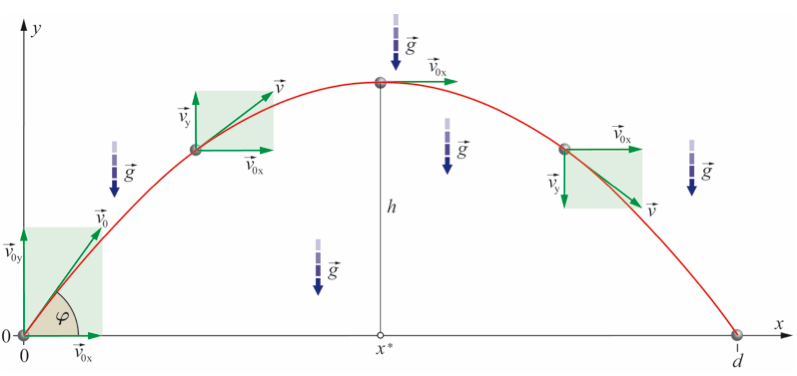
\includegraphics[width=0.9\linewidth]{images/schiefer_wurf}
\end{minipage}
\hfill
\begin{minipage}[h!]{0.4\linewidth}
Bahngleichung des Schiefen Wurfs: 
\begin{align*}
y = x \cdot tan(\varphi) - \frac{g x^2}{2 v_0^2 \cos^2(\varphi)}
\end{align*}
\end{minipage}

\begin{tabbing}
	\begin{tabu} to \linewidth {X l X l}
		\toprule
		Strecke in X & $s_x = v_0 t \cos(\alpha)$ &
		Strecke in Y & $s_y = v_0 t \sin(\alpha)  - \frac{gt^2}{2}$ \\
		Maximale Wurfhöhe & $y_{max} = \frac{v_0^2 \cdot \sin^2(\alpha)}{2g}$ &
		Maximale Wurfweite & $d = \frac{v_0^2 \cdot \sin(2\alpha)}{g}$ \\
	\end{tabu}
\end{tabbing}

\begin{tabbing}
	\begin{tabu} to \linewidth {l X}
		Momentan Geschwindigkeit & $v(t) = \sqrt{v_0^2 + g^2 t^2 - 2 v_0 \sin(\alpha) gt}$ \\
		Distanz bis zur maximale Höhe & $x_{ymax} = \frac{v_0^2 \sin^2(\alpha) \cos(\alpha)}{g} = \frac{d}{2}$ \\
		Y für bekanntes X & $y = \tan(\alpha) \cdot x - \frac{g}{2 \cdot v_0^2 \cos^2(\alpha)} \cdot x^2 $ \\
		Horizontale Geschwindigkeit & $v_x = v_0 \cdot cos(\alpha)$ \\
		Vertikale Geschwindigkeit & $v_y = v_0 \cdot sin(\alpha) - g t$ \\
	\end{tabu}
\end{tabbing}

\begin{tabbing}
	\begin{tabu} to \linewidth {l X l}
		Variable & Bedeutung & SI-Einheit \\
		\midrule
		$\alpha$ & Abwurfwinkel & $\text{Grad}^\circ$ \\ 
		$g$ & Fallbeschleunigung  & $\frac{m}{s^2}$  \\ 
		$v_0$ & Betrag der Anfangsgeschwindigkeit & $\frac{m}{s}$ \\ 
		$t$ & Zeit & $s$ \\ 
		\bottomrule
	\end{tabu}
\end{tabbing}


\vfill\null
\columnbreak

\paragraph{Senkrechter Wurf und Horizontaler Wurf} \hfill \\

\begin{itemize}
	\item Beim senkrechten Wurf gelten die Formeln des Schiefen Wurfs mit dem Winkel $\varphi = 90^\circ$
	\item Beim horizontale Wurf gelten die Formeln des Schiefen Wurfs mit dem Winkel $\varphi = 0^\circ$
\end{itemize}

\begin{minipage}[h!]{0.5\linewidth}
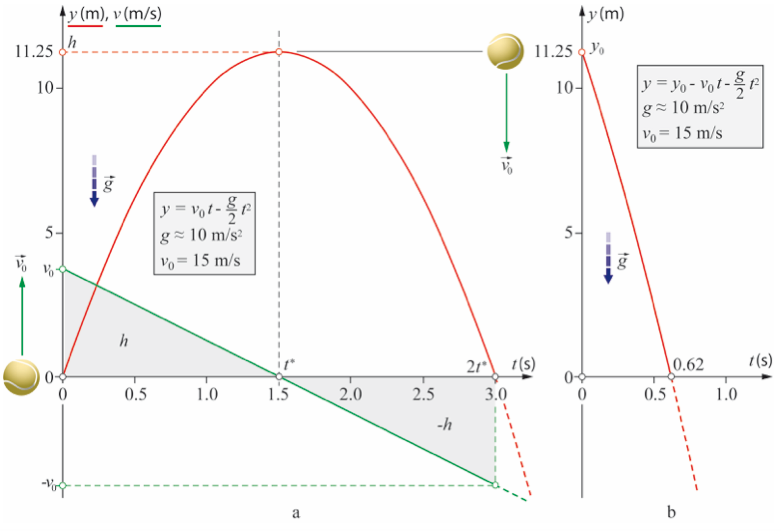
\includegraphics[width=0.9\linewidth]{images/senkrechter_wurf}
\end{minipage}
\hfill
\begin{minipage}[hbt]{0.5\linewidth}
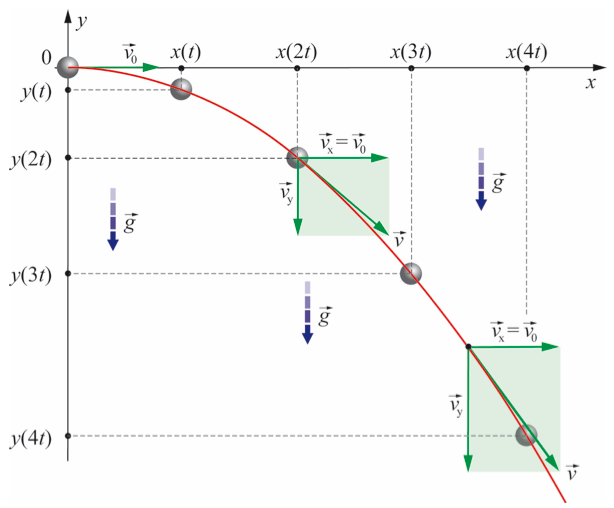
\includegraphics[width=0.9\linewidth]{images/horizontaler_wurf}
\end{minipage}

